\chapter{Optimierung}
\section{Jagen der Beute}
Ratten jagen in der Gruppe und es kommt ihr Sozialverhalten zum Tragen. Mathematisch wird dies dadurch abgebildet, dass eine Ratte als Schwarmführer fungiert und alle anderen Ratten dieser folgen. Als Schwarmführer nimmt man die beste bisherige Lösung, zu der alle anderen Mitglieder des Schwarmes hin konvergieren. \\
Hierzu werden folgende Formeln angenommen: 
\begin{equation}
    \vec{P} = A \cdot \vec{P_i}(x) + C \cdot (\vec{P_r}(x) - \vec{P_i}(x))
    \label{calcP}
\end{equation}
\begin{equation}
    A = R-x \cdot (\frac{R}{Max_Iteration})
    \label{calcA}
\end{equation}
\begin{equation}
    C = Random \in [0,2]
    \label{calcC}
\end{equation}
\begin{equation}
    R = Random \in [1,5]
    \label{calcR}
\end{equation}
Der Vektor $\vec{P_i}(x)$ steht dabei für die Position einer Ratte im Schwarm und der Vektor $\vec{P_r}(x)$ bildet die Ratte mit der besten Lösung als Schwarmführer ab. $x$ steht für den Zähler der momentanen Iteration, der bis zur Grenze $Max_Iteration$ hochgezählt wird. \\
$R$ und $C$ bilden Zufallszahlen ab, die für eine bessere Verteilung der einzelnen Ratten im Schwarm über die Dauer der Iterationen sorgen.

\section{Kampf mit der Beute}
Für den Kampf mit der Beute müsse sich die Ratten auf die Beute zu bewegen, was durch die folgende Formel ausgedrückt wird: 
\begin{equation}
    \vec{P_i}(x+1) = |\vec{P_r}(x) - \vec{P}|
    \label{calcPNext}
\end{equation}
$\vec{P_i}(x+1)$ steht dabei für die nächste Position einer einzelnen Ratte im Schwarm und richtet sich anhand der Position des Schwarmführers, der die beste bisherige Lösung abbildet, aus.\\
\autoref{rso_pos} zeigt die Verteilung der Ratten um die Beute. Durch Veränderung der Parameter $A$ und $C$ (siehe \autoref{calcA} und \autoref{calcC}) kann die Position einer Ratte auf alle abgebildeten Positionen verändert werden. \\ 
Die optimale Lösung wird im Algorithmus der 'Rat Swarm Optimization' mit den möglichst wenigen Operatoren gespeichert, was diesen Algorithmusmus sehr schlank und leichtgewichtig bei gleichzeitig sehr großer Effizienz und Konvergenz hin zum Optimum macht.\\
Der zu diesem Algorithmus zugehörige Pseudocode ist unter \autoref{rso_pseudocode} zu finden.
\begin{figure}[ht]
    \begin{center}
        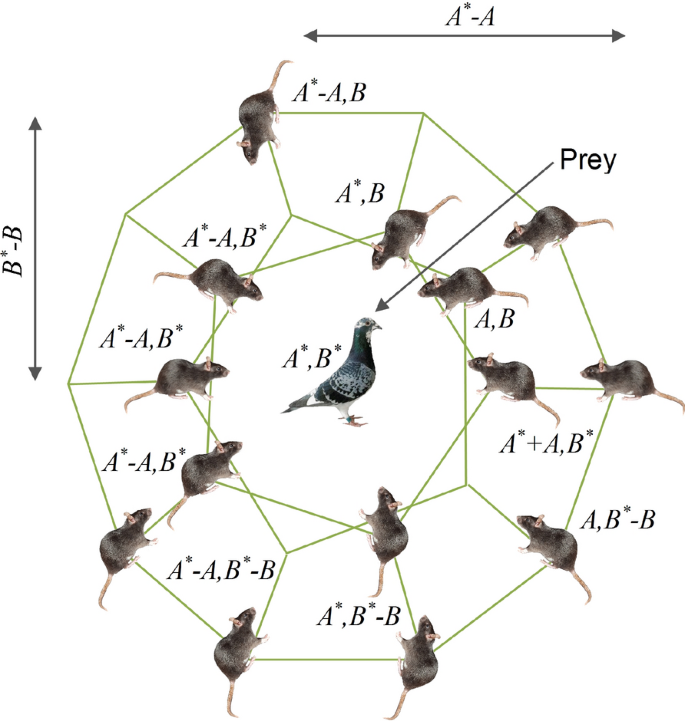
\includegraphics[width=0.7\textwidth]{assets/img/12652_2020_2580_Fig1_HTML.png}
        \caption[Positionsverteilung der Ratten im Schwarm um die Beute]{Positionsverteilung der Ratten im Schwarm um die Beute \cite{dhiman_garg_nagar_kumar_dehghani_2020}}
        \label{rso_pos}
    \end{center}
\end{figure}

\begin{figure}[ht]
    \begin{center}
        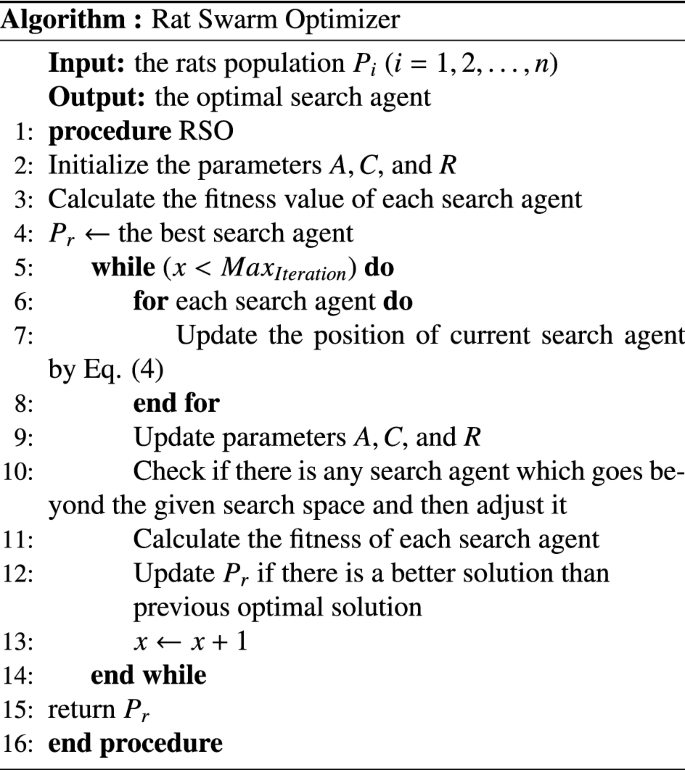
\includegraphics[width=0.7\textwidth]{assets/img/12652_2020_2580_Figa_HTML.png}
        \caption[Pseudocode RSO]{Pseudocode RSO \cite{dhiman_garg_nagar_kumar_dehghani_2020}}
        \label{rso_pseudocode}
    \end{center}
\end{figure}